\section{Portrait and landscape}\label{sec:orientation}

The stand is set up for \textbf{portrait}. The mount was raised so that a 488\,mm tall screen still clears the
base by 56\,mm. The VESA pattern is square, so changing orientation never touches the stand: only the four M4
screws come out.

\begin{figure}[H]
  \centering
  \begin{subfigure}{0.49\linewidth}\centering
    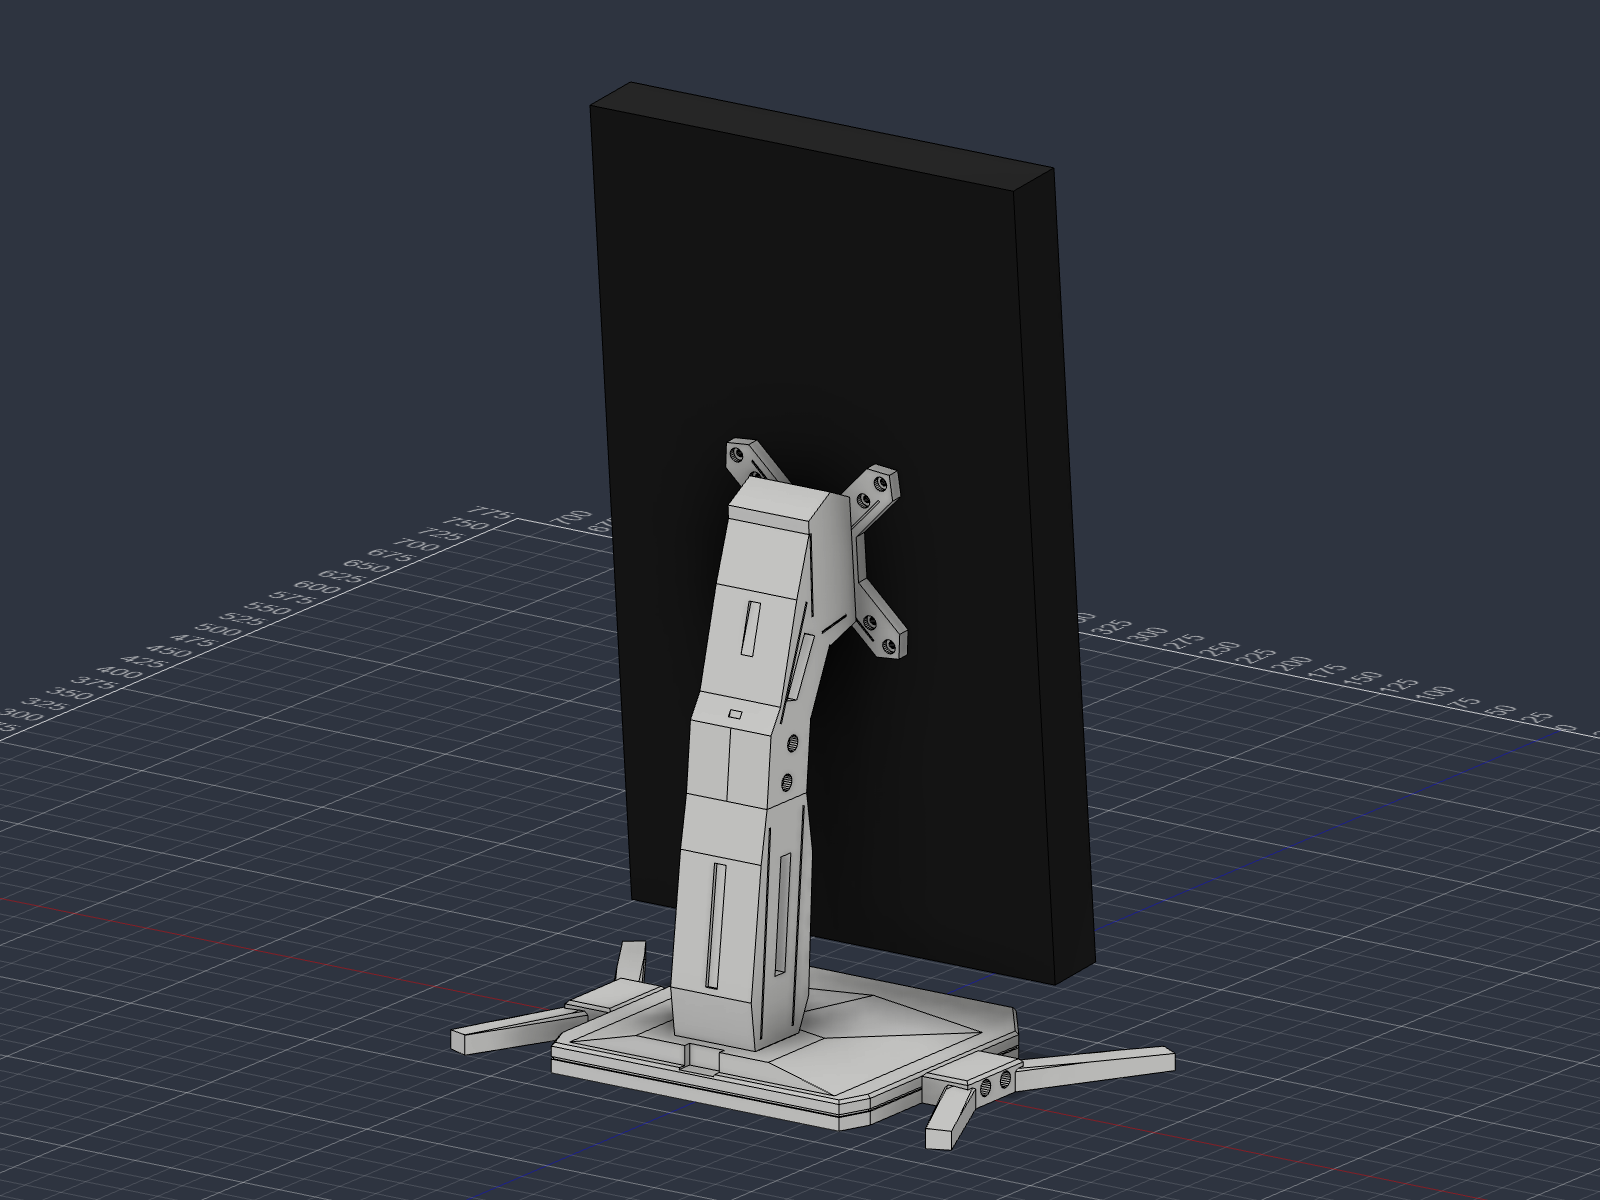
\includegraphics[width = \linewidth]{with-monitor-portrait.png}\caption{Portrait (daily use).}
  \end{subfigure}\hfill
  \begin{subfigure}{0.49\linewidth}\centering
    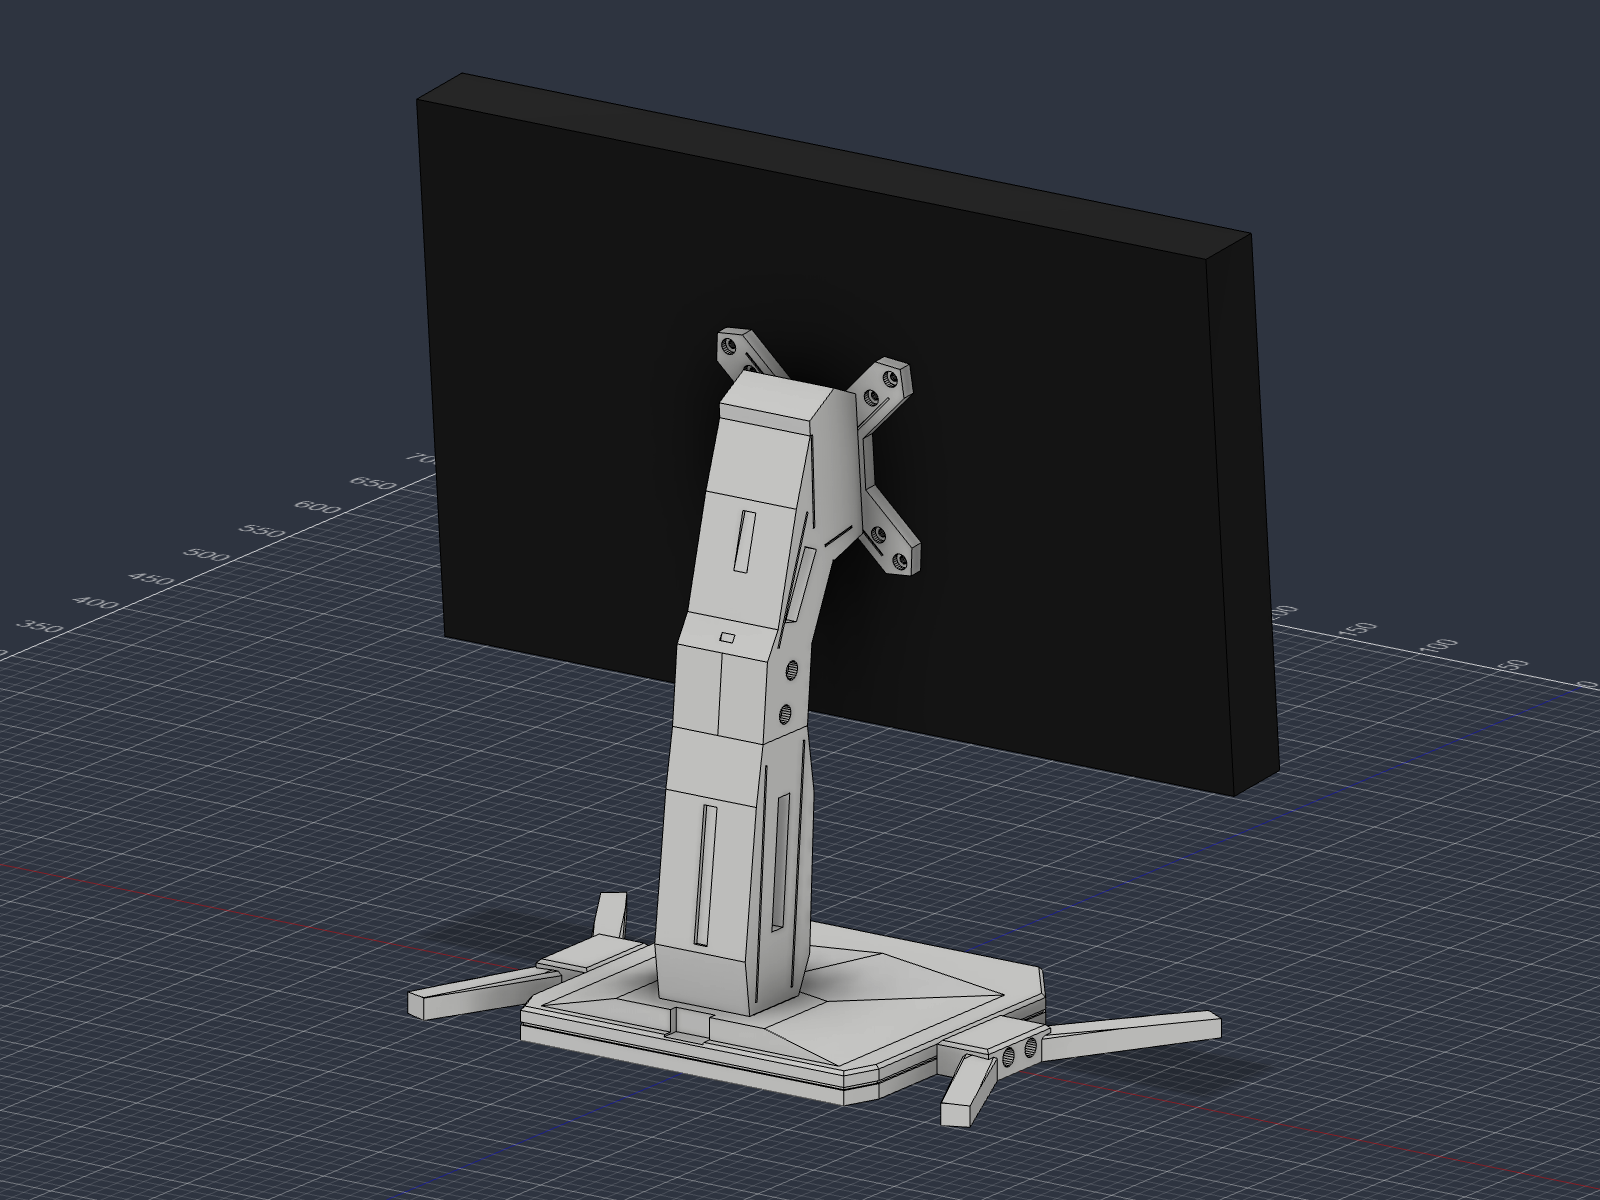
\includegraphics[width = \linewidth]{with-monitor-landscape.png}\caption{Landscape.}
  \end{subfigure}
  \caption{Both orientations use the same plate holes.}
\end{figure}

\begin{step}{Switching orientation (about 2 minutes)}
\begin{enumerate}
  \item Turn the monitor off and unplug the cables from it, or leave enough slack for a 90° turn.
  \item Support the monitor with one hand. With the other, remove the four \textbf{M4} screws from behind the plate.
  \item Rotate the monitor 90°. In portrait, turn it so the cable ports end up on the side closer to the cable window.
  \item Hold it against the plate and drive the four M4 screws back in, starting all four before tightening.
  \item Rotate the image: on macOS, \emph{System Settings → Displays → Rotation}; on Windows, \emph{Settings → System →
        Display → Display orientation}.
\end{enumerate}
\end{step}

\begin{nota}
If you switch often, keep the M4 screws in a small magnetic tray, and do not over-tighten them: the threads are in the
monitor, not in the print.
\end{nota}
